\chapter{Generating Exponential Random Variables}

\setcounter{problem}{1}
\section{Discussion}

\begin{fullwidth}

The goal of this lab is to generate random values from the exponential distribution using the inverse transform method.  You will show the histogram of the random values and then show the theoretical exponential distribution on top to verify your results. We will need the statistics stuff from {\bf scipy} to get the theoretical exponential distribution. Use filename {\tt rexp.py}.

\section{Steps}

\step First, creative function called {\tt rexp(lambduh)} that returns a random value from an exponential distribution. Look up the inverse of the exponential cumulative distribution function in Wikipedia.

\begin{pyverbatim}
def rexp(lambduh): # lambduh mispelled to avoid clash with lambda in python
    # u = get value from U(0,1)
    # return F^-1(u) for exp cdf
\end{pyverbatim}

\step You will need the usual libraries plus scipy:

\begin{pyverbatim}
import math
import matplotlib.pyplot as plt
import numpy as np
import scipy.stats as stats
\end{pyverbatim}

\step Get a sample of exponential random variables from $Exp(1.5)$ in variable {\tt X} (see code from previous lab); I usually define constants to make the code more readable:

\begin{pyverbatim}
N = 1000
LAMBDUH = 1.5
\end{pyverbatim}

\step Display a histogram using matplotlib (in a separate window)

\begin{pyverbatim}
plt.hist(y, bins=20, normed=1) # use bins option to get better resolution
plt.show()
\end{pyverbatim}

\step Run it. You should see something like this:

\scalebox{.35}{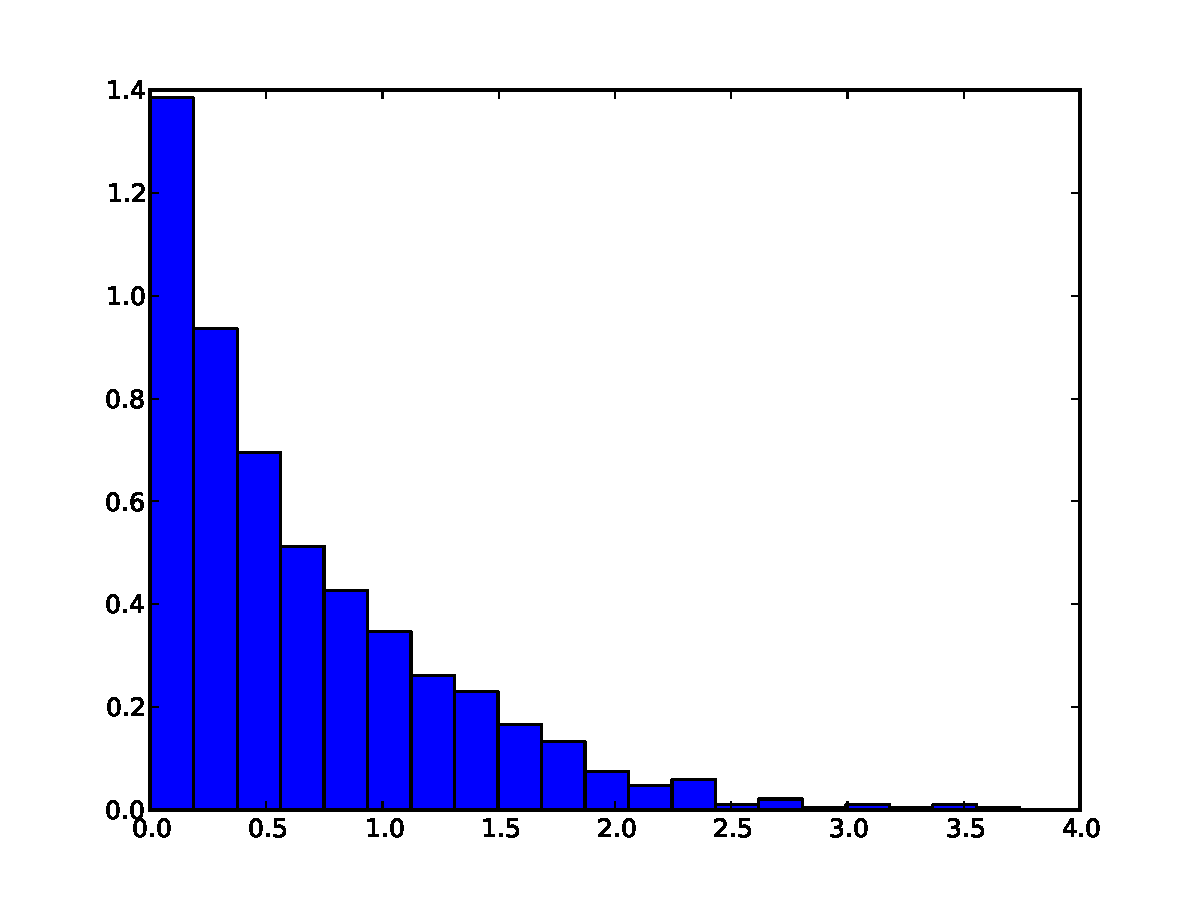
\includegraphics{figures/exp-1_5-density.pdf}}

{\bf How do we know that this accurately represents the exponential distribution? We plot the theoretical distribution on top with a red line.}\\

\step Before the {\tt show()}, do this (yes, we have two plot() calls now):

\begin{pyverbatim}
# Show real distribution
x = np.arange(0,6, 0.01) # get a set of values from 0..6 stepping by 0.01
y = stats.expon.pdf(x, scale = 1.0/LAMBDUH) # pdf takes 1/lambda not lambda
plt.plot(x,y, color='red')
\end{pyverbatim}

\step Run it.  You should see the following.\\

\scalebox{.35}{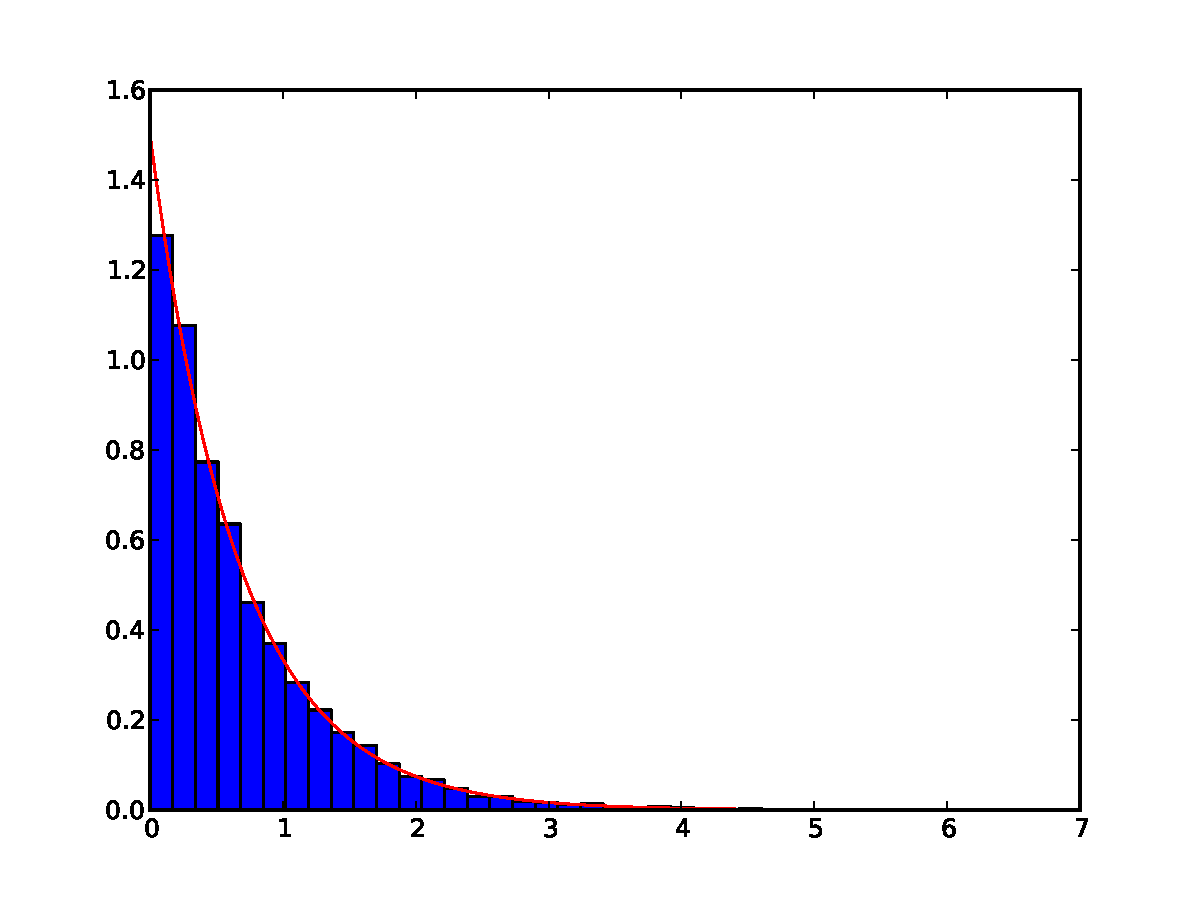
\includegraphics{figures/exp-1_5-density-fancy.pdf}}

\section{Deliverables}

Please submit:

\begin{itemize}
\item your Python file
\item a PDF of your final graph.
\end{itemize}

\end{fullwidth}
